% !TeX program = xelatex
\documentclass[a4paper,14pt]{extarticle} % Использование extarticle для 14pt шрифта
\usepackage{fontspec} % Для использования системных шрифтов	
\usepackage{polyglossia} % Для многоязыковой поддержки
\usepackage{amsmath}
\usepackage{amsfonts}
\usepackage{amssymb}
\usepackage{listings}
\usepackage{xcolor}
\usepackage{indentfirst} % Для отступа в первом абзаце
\setlength{\parindent}{1.25cm} % Установка отступа в 1.25 см
\setlength{\parskip}{0em} % Установка межабзацного интервала в 0

\newfontfamily\cyrillicfonttt{Courier New}

\lstset{ 
    language=[Sharp]C,              % Язык кода - C#
    basicstyle=\ttfamily\footnotesize, % Основной стиль шрифта
    keywordstyle=\color{blue},       % Цвет ключевых слов
    commentstyle=\color{green},      % Цвет комментариев
    stringstyle=\color{red},         % Цвет строк
    numbers=left,                   % Номера строк слева
    numberstyle=\tiny\color{gray},  % Стиль номеров строк
    stepnumber=1,                   % Нумерация каждой строки
    numbersep=5pt,                  % Расстояние между номерами строк и кодом
    showspaces=false,               % Показывать пробелы
    showstringspaces=false,         % Показывать пробелы внутри строк
    showtabs=false,                 % Показывать табуляцию
    frame=single,                   % Рамка вокруг кода
    tabsize=4,                      % Размер табуляции
    captionpos=b,                   % Позиция заголовка (b - снизу)
    breaklines=true,                % Перенос строк
    breakatwhitespace=false,        % Переносить строки только на пробелах
    title=\lstname,                 % Показывать название файла
    escapeinside={\%*}{*)},         % ЛаТеХ команды внутри кода
    morekeywords={var, get, set}    % Дополнительные ключевые слова
}

\renewcommand{\lstlistingname}{Лістинг} % Зміна підпису лістингу на українську мову

\setmainlanguage{ukrainian} % Основной язык документа
\setotherlanguage{english} % Дополнительный язык документа
\setmainfont{Times New Roman} % Установка шрифта Times New Roman
\usepackage{geometry} % Пакет для настройки полей страницы
\geometry{
    left=3cm,
    right=1.5cm,
    top=2cm,
    bottom=2cm
}

\usepackage{titlesec} % Пакет для настройки заголовков
\titleformat{\section}{\large\bfseries}{\thesection}{1em}{}
\titleformat{\subsection}{\normalsize\bfseries}{\thesubsection}{1em}{}

\usepackage{setspace} % Пакет для настройки межстрочного интервала
\onehalfspacing % Установка полуторного интервала

\usepackage{tocloft} % Пакет для настройки оглавления
\renewcommand{\cftsecleader}{\cftdotfill{\cftdotsep}} % Добавление точек к оглавлению

\usepackage{fancyhdr} % Пакет для настройки колонтитулов
\pagestyle{fancy}
\fancyhf{}
\fancyfoot[C]{\thepage}
\renewcommand{\headrulewidth}{0pt} % Убирает линию вверху страницы
\renewcommand{\footrulewidth}{0pt} % Убирает линию внизу страницы

\usepackage{graphicx}
\usepackage{caption} % Пакет для підписів до зображень
\usepackage{hyperref} % Пакет для создания кликабельных ссылок

\begin{document}	

    % Титульная страница
    \begin{titlepage}
        \centering
        \large
        Київський нацiональний унiверситет iменi Тараса Шевченка\\
        Факультет комп’ютерних наук та кiбернетики\\
        Кафедра математичної інформатики\\
        
        \vspace*{4cm}
        
        \huge Курсова робота на тему: \\
            \textbf{Розробка методики порівняння ефективності алгоритмів патерн-метчингу}
        
        \vspace{4cm}
        
        \raggedleft
        \large
        \begin{tabular}{r}
            Виконав студент 3 курсу \\
            Гришечкін Тихон Сергійович \\
            \\
            Науковий керівник: \\
            доцент, доктор фізико-математичних наук Завадський І.О \\
        \end{tabular}
        
        \vfill
        
        \centering
        \large
        Київ, 2024
        
    \end{titlepage}
    
    % Оглавление
    \tableofcontents
    \newpage
    
    % Вступ
    \section{Вступ}

	Задача пошуку рядку є важливою задачею в інформатиці. Вона має широке застосування в різних областях, зокрема:

\begin{itemize}
    \item Інформаційний пошук: Алгоритми пошуку рядків використовуються в пошукових системах для
	знаходження релевантних документів на основі запитів користувачів.
    \item Біоінформатика: Пошук підрядків є ключовим у знаходженні послідовностей нуклеотидів або амінокислот у геномах та протеомах. \cite{dna}
    \item Обробка текстів: Алгоритми пошуку використовуються для знаходження та заміни текстових фрагментів у текстових редакторах.
    \item Бази даних: Пошук підрядків використовується в базах даних для виконання запитів зі згадками текстових фрагментів або шаблонів.
    \item Компіляція: Компілятори використовують алгоритми пошуку підрядків для аналізу та оптимізації програмного коду.

\end{itemize}

Тому важливою задачею є оцінка ефективності цих алгоритмів. Оцінка ефективності дозволяє визначити, який з алгоритмів найкраще підходить для конкретних умов та обмежень. У даній курсовій роботі ми запропонуємо методику порівняння ефективності різних алгоритмів пошуку рядку. Ми проведемо експериментальне дослідження на основі ряду критеріїв, таких як швидкість виконання, та стійкість до різних типів вхідних даних.

Результати даного дослідження можуть бути корисними для вибору оптимального алгоритму в залежності від конкретної задачі та умов її виконання.


    \newpage



    % Основна частина
    \section{Алгоритми пошуку рядка}

	\subsection{Постановка задачі патерн-метчингу}

	Нехай дані дві послідовності: текст \( T \) та патерн \( P \) (далі також інколи позначається, як <<шаблон>>), де \( |T| = n \) та \( |P| = m \). Задача полягає у знаходженні всіх входжень патерна \( P \) у текст \( T \).

При цьому передбачається, що:
\begin{itemize}
    \item \( T \) та \( P \) складаються з символів алфавіту \( \Sigma \).
    \item Алфавіт \( \Sigma \) може бути скінченним або нескінченним, але у нашій постановці розглядається скінченний алфавіт.
\end{itemize}


Розглядається задача пошуку підстроки у формулюванні \textbf{single-pattern matching}, що передбачає пошук одного заданого патерна в тексті. Не розглядаються задачі \textbf{approximate pattern searching}, де потрібно знаходити патерни з певною степенню схожості, або \textbf{regular pattern searching}, де патерн може бути виражений у вигляді регулярного виразу.


	\subsection{Загальна характеристика алгоритмів пошуку рядка}

	Найпростішим методом для пошуку підрядка в рядку є алгоритм повного перебору (brute force). Його суть полягає у перевірці кожної позиції в тексті \( T \) як можливої початкової позиції для патерна \( P \). Для кожної такої позиції перевіряється, чи співпадає патерн \( P \) з відповідною підстрокою в тексті \( T \). Цей метод має часову складність \( O(n \cdot m) \), де \( n \) – довжина тексту, а \( m \) – довжина патерна. Через високу обчислювальну складність цей алгоритм є дуже неоптимальним для великих текстів і патернів.

	У 1970 році Д. Морріс та В. Пратт \cite{morris-pratt} розробили перший оптимальний алгоритм пошуку підстроки – алгоритм Кнута-Морріса-Пратта (KMP). Цей алгоритм значно покращив ефективність пошуку, зменшивши часову складність до \( O(n + m) \).

	З часом з'явилося багато інших алгоритмів (більше 124 див. \cite{smart}). Всі ці алгоритми можна умовно поділити на чотири основні категорії:
	\begin{itemize}
		\item алгоритми на основі порівняння символів
		\item  алгоритми на основі суфіксних автоматів
		\item алгоритми на основі побітового паралелізму
		\item гібридні алгоритми.
	\end{itemize}

\textbf{Алгоритми на основі порівняння символів}

Алгоритми на основі порівняння символів (Character-based approaches) є класичним підходом, який просто порівнює символи для вирішення задач пошуку рядка.

Алгоритми на основі порівняння символів мають дві основні стадії: пошук і зсув. Алгоритм Бойера-Мура \cite{bm}, є стандартним та еталонним методом цього типу. Він використовує таблицю зсувів для пропуску непотрібних порівнянь, що значно підвищує швидкість пошуку.

\textbf{Алгоритми на основі суфіксних автоматів}

Суфіксний автомат (Suffix automaton) складається з детермінованого ациклічного кінцевого автомата та суфіксного автомата, які разом дозволяють ефективно здійснювати пошук рядка.

Цей метод використовує спрямований ациклічний граф, де вершини є станами, а ребра – переходами між станами. Суфіксний автомат розпізнає всі суфікси патерна і дозволяє швидко знаходити підрядки.
Прикладом алгоритму даного класу є є Backward-DAWG-Matching алгоритм (BDM).

\textbf{Алгоритми на основі побітового паралелізму}

Алгоритми на основі паралелізму бітового рівня були запропоновані для прискорення процесу пошуку шляхом використання внутрішнього паралелізму бітових операцій, що зменшує кількість операцій у рази до $\omega$, де $\omega$ –  кількость бітів у машинному слові.

Ці алгоритми є швидкими та ефективними, особливо коли довжина патерна менша за довжину машинного слова. До таких алгоритмів належать наприклад Shift-OR (SO), Shift-AND (SA) алгоритми.

\textbf{Гібридні алгоритми}

Гібридні алгоритми комбінують переваги різних методів для вирішення складних задач. Вони поєднують методи з різних категорій для досягнення кращої ефективності.

Таким чином, за роки розвитку цієї області задач з'явилося багато алгоритмів для пошуку підрядка, які можна класифікувати за чотирма основними категоріями. Кожен клас алгоритмів має свої недоліки та переваги, які важливо розуміти при виборі оптимального алгоритму для своєї задачі.

\subsection{Алгоритм Бойера-Мура}
Розглянемо детальніше деякі алгоритми пошуку.

Першим розглянемо алгоритм Бойера-Мура (BM), який є класичним представником класу <<character-based>> алгоритмів.

Алгоритм шукає входження патерну $\textbf{p}$, прикладаючи його до тексту $\textbf{t}$ зліва направо, але при цьому порівняння, виконаються справа наліво, починаючи з останнього символу патерну.

Далі якщо при порівнянні знайдено перший неспівпадаючий символ патерну, то виконується зсув патерну на деяку кількість позицій, за допомогою наступних евристик:

\begin{itemize}
	\item \textit{Евристика стоп символів}:
	
	Для цього для кожного символу алфавіту $\Sigma$ запам'ятовуємо індекс останнього його входження в патерн, якщо він є, або запам'ятовуємо -1, якщо він не входить в патерн (вважаємо, що індексація символів починається з нуля). 
	Назвемо цей масив індексів $StopTable$.
	
	Тепер розглянемо символ тексту $c$, що не співпав на поточній ітерації порівняння. Позначимо поточний індекс патерну на якому відбулось неспівпадіння як $i$.
	Тоді якщо виконується \[i-StopTable[c] > 0\] то відбувається зсув патерну на $i-StopTable[c]$ кроків, інакше кажучи на найменшу кількість кроків щоб відбулось співпадіння з символом $c$. (рис. \ref{fig:boyer_moore})
	\item \textit{Евристика співпадаючого суфікса}:
	
	Якщо при порівнянні шаблону справа наліво збігся суфікс \( S \), а символ \( c \), що стоїть перед \( S \) в шаблоні не збігся (тобто шаблон має вигляд \( PcS \)),
 	то евристика співпадаючого суфікса зсуває шаблон на найменше число позицій вправо так, щоб рядок \( S \) збігся з шаблоном, а символ, що передує даному збігу \( S \) в шаблоні, відрізнявся б від \( c \).
	
	Заради цього для патерну $p$ перед початком пошуку, обраховуються відповідні величини зсуву, за допомогою алгоритму,
	схожого за ідеєю на алгоритми обчислення <<префікс-функції>> та <<Z-функції>>.

	Як і випадку цих алгоритмів ці зсуви обчислюються за $O(m)$ операцій.
	
	Далі в алгоритмі просто використовуються ці заздалегідь обчислені зсуви при неспівпадінні символів.

	Зазначимо, що якщо на кожній ітерації просто знову порівнювати символи, навіть з використанням зсувів асимптотика алгоритму
	складає $O(n*m)$ операцій. Для досягнення складності $O(n+m)$, треба не порівнювати з шаблоном вже співпадаючий суфікс, знайдений на попередній ітерації.

\end{itemize}
	\begin{figure}[h] % Починаємо середовище figure
		\centering % Центруємо малюнок
		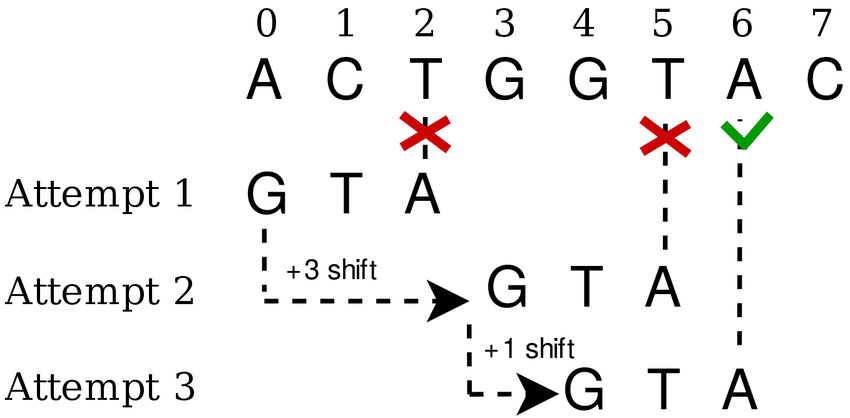
\includegraphics[width=0.6\textwidth]{images/boyer_moore.png} % Вставляємо малюнок
		\caption{Приклад використання евристики стоп символів} % Підпис до малюнка
		\label{fig:boyer_moore} % Мітка для посилань на малюнок
	\end{figure}
	\begin{figure}[h] % Починаємо середовище figure
		\centering % Центруємо малюнок
		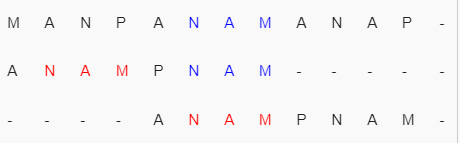
\includegraphics[width=0.6\textwidth]{images/boyer_moore_suffix.png} % Вставляємо малюнок
		\caption{Приклад використання евристики співпадаючого суфікса} % Підпис до малюнка
		\label{fig:boyer_moore_suffix} % Мітка для посилань на малюнок
	\end{figure}

    \newpage
	Додамо також, що існує багато модифікацій алгоритму Бойера-Мура, які використовують інші евристики або реалізують вже існуючі інакше.
	
	Прикладами таких алгоритмів є алгоритми Бойєра - Мура - Хорспула (BMH), Чжу - Такаокі (ZT), турбо - Бойера - Мура (TBM).

	Наприклад BMH використвує тільки <<евристику стоп символів>>, але тільки за останнім символом, тому є спрощени варіантом Бойера-Мура.

	ZT використовує також <<евристику стоп символів>>, але для пар символів, заради оптимізації при маленьких алфавітах.

	\subsection{Алгоритми Shift-OR (SO) та Shift-AND (SA)}

	Розглянемо алгоритми Shift-OR (SO) та Shift-AND (SA), які є представниками класу алгоритмів основаних на паралелізмі бітових операцій.

	Опишемо SA алгоритм.

	Нехай маємо $i$-й символ тексту $t$. 

	Введемо матрицю $Mask$, де
	\[Mask[i][j] = 1,\text{якщо } t[i-j..i] = p[0..j]\]
	\[Mask[i][j] = 0,\text{якщо } t[i-j..i] \neq  p[0..j]\]

	Тоді маємо входження шаблону на $i$-му кроці, коли $Mask[i][m-1] = 1$.

	Але вичислення матриці $Mask$, на кожному кроці займає $O(m)$ операцій тому такий алгоритм нічим не краще <<Brute-Force>> алгоритму, і фактично ним і є.

	Тоді нехай маємо матрицю $pos$, де для символу $c$ маємо
	\[pos[c][j] = 1,\text{якщо } p[j]=c\]
	\[pos[c][j] = 0,\text{якщо } p[j] \neq c\]
	Можемо помітити наступну властивість. 
	$$Mask[i]=(Mask[i-1]<<1)\And pos[t[i]]$$

	Де $<<$ - операція побітового зсуву вліво.

	Тепер можемо в рамках реалізації замінити вектори $Mask[i]$ та $pos[c]$, на звичайні змінні, для яких всі операції будуть виконані $O(1)$, але отримаємо очевидне обмеження $m<\omega$, де $\omega$ - довжина машинного слова.

	Shift-or алгоритм аналогічний алгоритму Shift-and, де просто інвертовано вектори $Mask[i]$ та $pos[c]$, а операція $and$ замінюється на $or$. 
	А критерієм входження стає $Mask[i][m-1]=0$.

	Алгоритми, що основані на паралелізмі бітових операцій називаються так бо на кожному кроці виконується $\omega$ паралельних порівнянь, хоча фактично виконується лише декілька бітових операцій.

	Такі алгоритми дають значне прискорення на патернах невеликої довжини, для яких вони і були створені. Для $m>\omega$, зазвичай ці алгоритми оптимізують або об'єднують з іншими.

	Наприклад у SA, для патернів більшої довжини, при знаходженні співпадіння довжини $\omega$ решту символів просто перевіряють до першого неспівпадіння.

    % Практична частина
    \section{Практична частина}

    \newpage
    % Висновки
    \section{Висновки}

    \newpage
    
    % Список літератури
    \begin{thebibliography}{9}
        \addcontentsline{toc}{section}{Література} % Добавление списка литературы в оглавление
		\bibitem{dna}
		Alsmadi, I., \& Nuser, M. (2012). String matching evaluation methods for DNA comparison. International Journal of Advanced Science and Technology, 47(1), 13-32.
		\bibitem{morris-pratt}
		J. H. Morris, Jr and V. R. Pratt. A linear pattern-matching algorithm. Report 40, University of California, Berkeley, 1970.
		\bibitem{smart}
		Faro, S., Lecroq, T., Borzi, S., Di Mauro, S.,\& Maggio, A. (2016, August). The String Matching Algorithms Research Tool. In Stringology (pp. 99-111).
		\bibitem{exact}
		Faro, S.,\& Lecroq, T. (2013). The exact online string matching problem: A review of the most recent results. ACM Computing Surveys (CSUR), 45(2), 1-42.
		\bibitem{bm}
		R. S. Boyer and J. S. Moore. A fast string searching algorithm. Commun.
ACM, 20(10):762–772, 1977.
    \end{thebibliography}
    
\end{document}